\section{Overview} \label{sec:overview}
At a high level, the system is divided into three \emph{layers}:
\begin{description}
    \item[Presentation layer] It contains the two types of clients (mobile
    application and website) from which the citizens and authorities will access
    the service.
    \item[Application layer] It contains all the business logic to handle
    incoming data from the users and other external sources, to compute
    suggestions and satisfy queries coming from the presentation layer.
    Here a Web Server only provides \emph{static content} for the web
    application, while the \emph{dynamic data} is provided through a REST API
    which is shared between the mobile app and the web app.
    \item[Data layer] It is responsible for storing all the data needed by the
    system, ensure its persistence over time, even in case of failure, and to
    make it available to the application components.
\end{description}
Each layer sees the other layers as single entities, hiding the internal
replication and complexity. In particular the usage of a REST model for
client-server communication provides a high level of \emph{uncoupling} between
the two layers and allows for efficient \emph{replication} of the application
servers, which is a key point to achieve fault tolerance and scalability.

Figure \vref{fig:architecture_overview} shows an overview of the physical
architecture, where we can notice the high degree of replication in the
application layer and the need for \emph{load balancers} to manage the
replicas.
Regarding the database we chose a relational DBMS. Here the entire data-set
should be partitioned on different nodes which share a single manager, since a
fully-distributed solution is difficult to manage while having to guarantee the
ACID properties.
We also represented the two external data sources that the system needs to
access: the \emph{DMV Service} to validate licence plate numbers and the
\emph{Accident Data Service} provided by some municipalities and needed to
provide SmartSuggestions functionality.
Finally, we represented a logical overview of the network that connects the
various components, underlining the fact that all external communication
travels on the internet and also the need for firewalls to protect the internal
components (application and data layers) from malicious attacks.

\begin{figure}[ht]
    \centering
    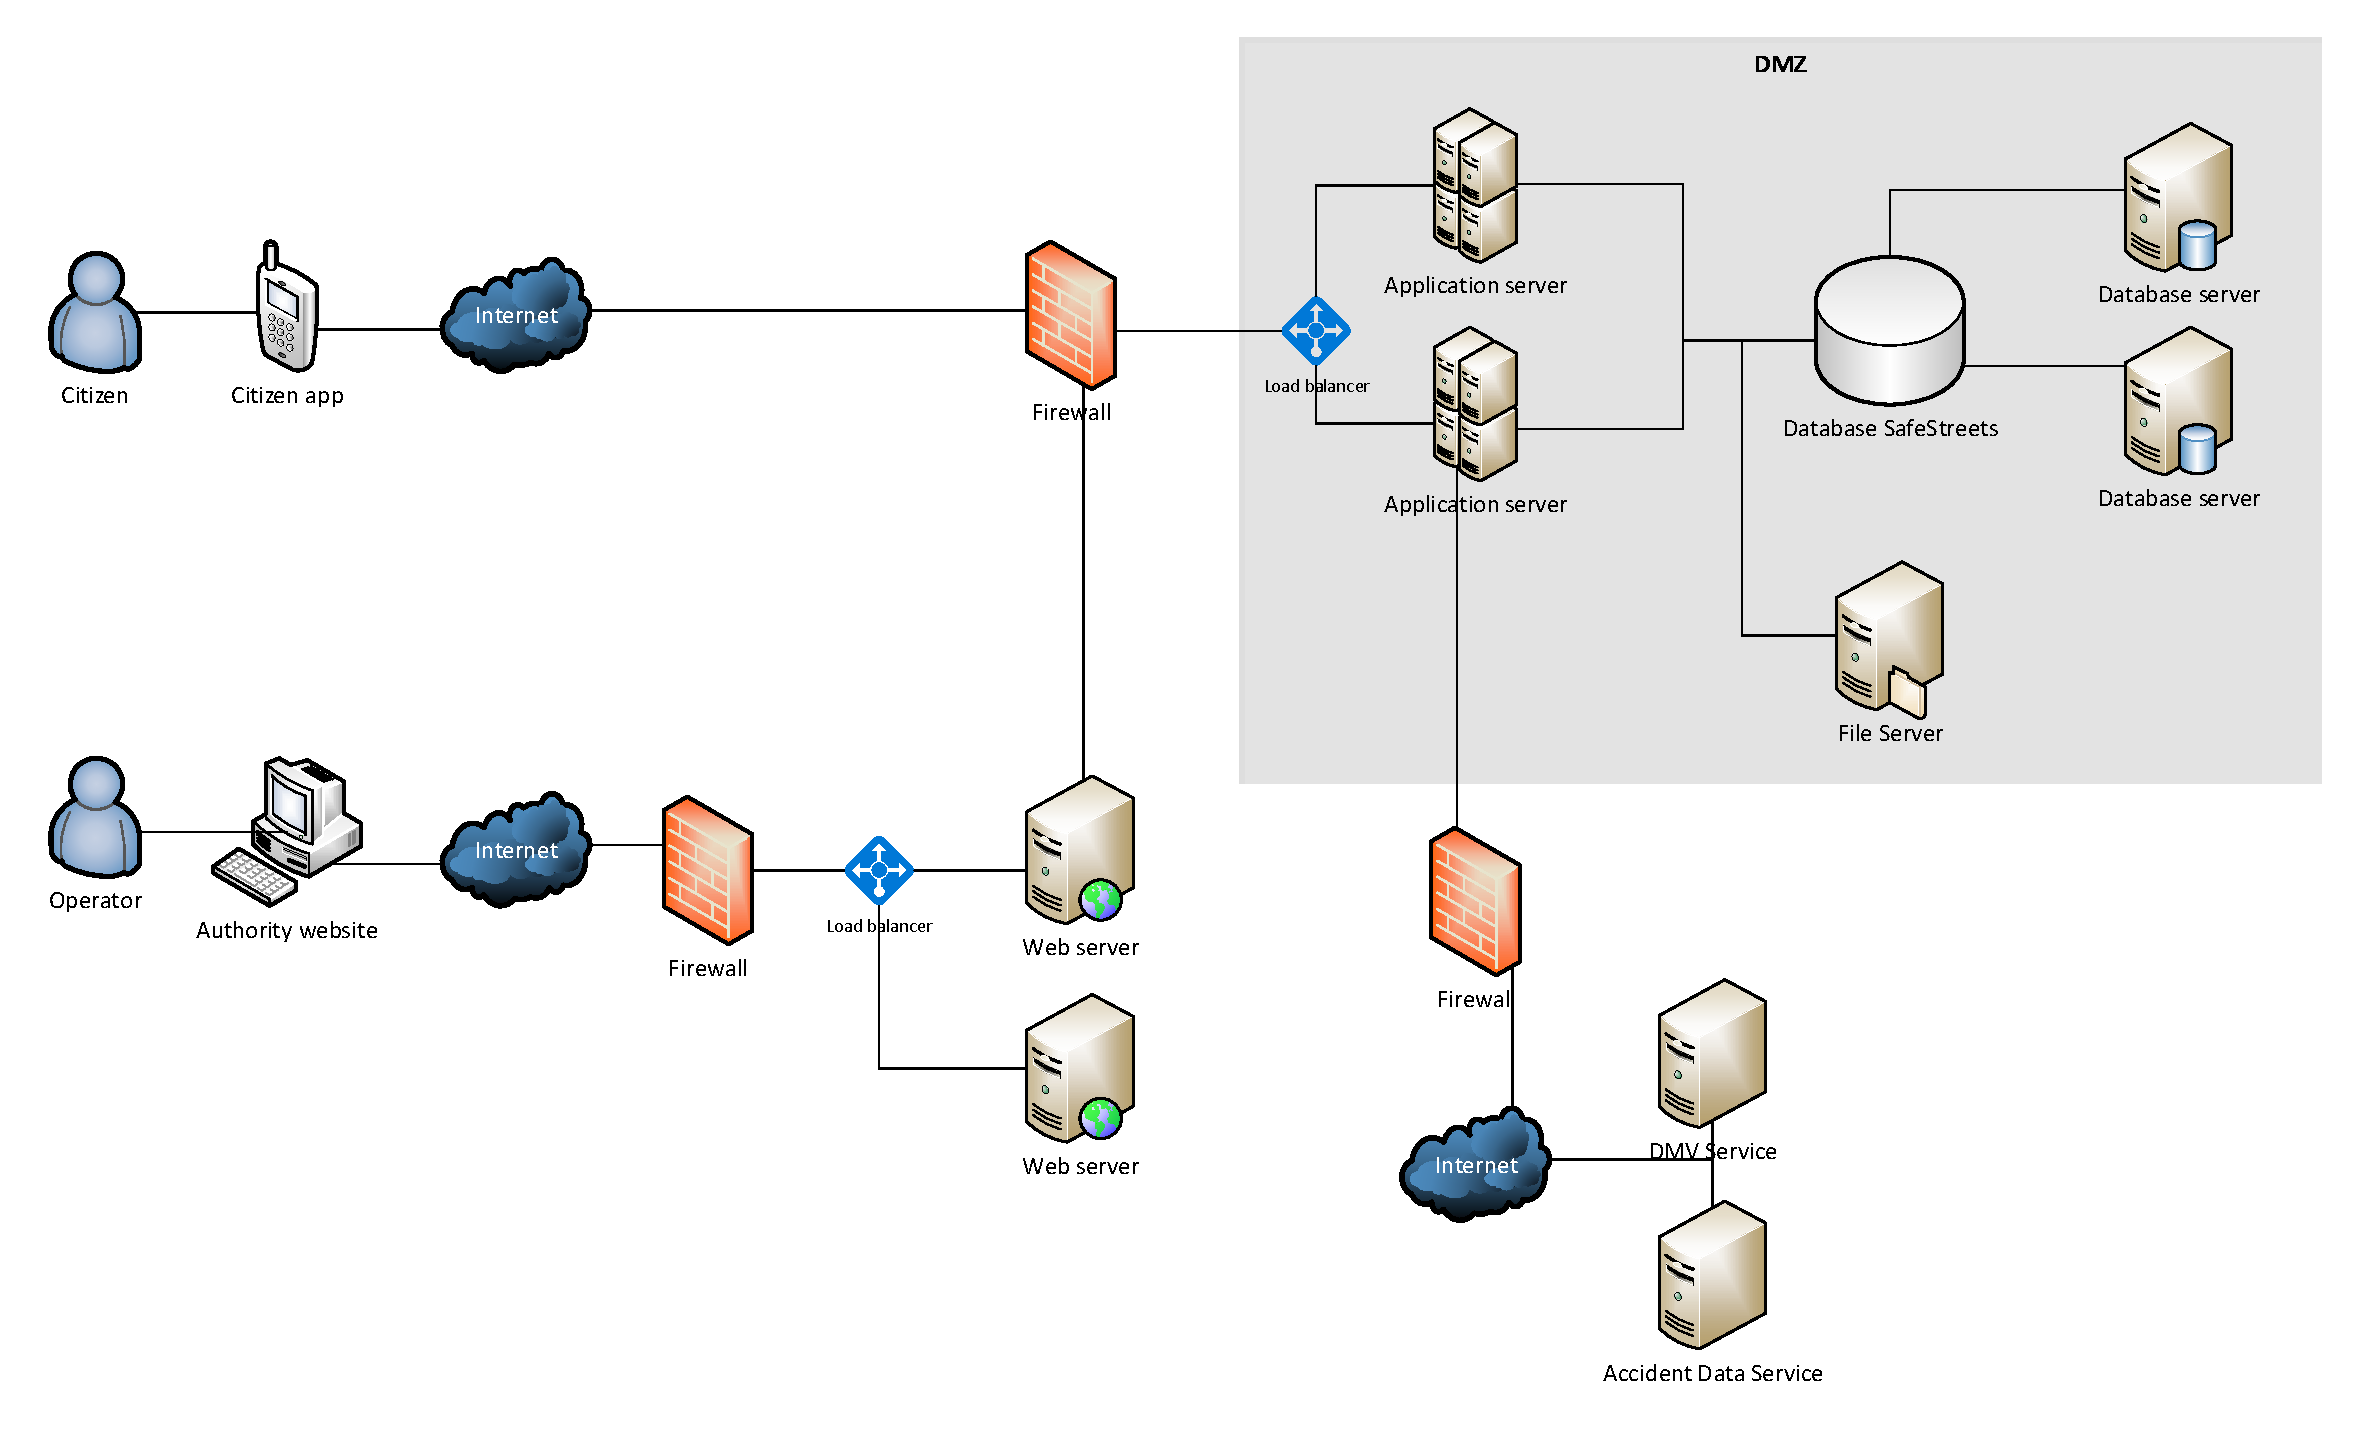
\includegraphics[width=\textwidth]{architecture_overview.pdf}
    \caption{Overview of the physical architecture}
    \label{fig:architecture_overview}
\end{figure}